%! TeX root = ../Parte2.tex

\section{Navigazione anonima}

\begin{myframe}{Modalità incognito}
  \begin{itemize}[<+->]
    \item Non salva la cronologia
    \item Cookie separati e temporanei
    \item Blocca alcuni tracker (solo su Firefox)
  \end{itemize}

  \pause\medskip
  Non offre quindi una protezione adeguata.
\end{myframe}

\begin{myframe}{Alternative}
  \begin{itemize}
    \item Proxy
    \item VPN
    \item Tor
  \end{itemize}
\end{myframe}

\begin{myframe}{Proxy}
  \begin{tikzpicture}[block/.style={draw, fill=yellow!20, shape=rectangle, minimum height=3em, minimum width=6em}]
    \node[block] (pc) {Dispositivo};
    \node[block, right=of pc] (proxy) {Proxy};
    \node[block, right=of proxy] (server) {Server};
    \onslide<2->{\draw[->] (pc.50) to[bend left] node[midway, above]{richiesta} (proxy.130);}
    \onslide<3->{\draw[->] (proxy.50) to[bend left] node[midway, above]{richiesta} (server.130);}
    \onslide<4->{\draw[->] (server.230) to[bend left] node[midway, below]{risposta} (proxy.310);}
    \onslide<5->{\draw[->] (proxy.230) to[bend left] node[midway, below]{risposta} (pc.310);}
  \end{tikzpicture}

  \medskip
  \onslide<6->{Il server vedrà il proxy, ma non il nostro dispositivo.}

  \onslide<7->{Purtroppo la connessione dal nostro dispositivo al proxy è visibile.}
\end{myframe}

\begin{myframe}{Virtual private network}
  \begin{tikzpicture}[block/.style={draw, fill=yellow!20, shape=rectangle, minimum height=3em, minimum width=6em}]
    \node[block] (pc) {Dispositivo};
    \node[block, right=of pc, text width=15em, align=center] (vpn) {VPN};
    \node[block, right=of vpn] (server) {Server};
    \onslide<2->{\draw[->] (pc.20) -- node[near start, above, yshift=.5em]{richiesta} (server.160);}
    \onslide<3->{\draw[->] (server.200) -- node[near start, below, yshift=-.5em]{risposta} (pc.340);}
  \end{tikzpicture}

  \medskip
  \onslide<4->{La VPN ci maschera come un proxy}

  \onslide<5->{ed inoltre la nostra connessione verso la VPN è criptata.}
\end{myframe}

\begin{myframe}{Rete TOR}
  \begin{tikzpicture}[block/.style={draw, fill=yellow!20, shape=rectangle, minimum height=3em, minimum width=6em},node/.style={draw, fill=yellow!20, shape=circle, minimum height=2em, minimum width=2em}]
    \node[block] (pc) {Dispositivo};
    \node[node, right=of pc] (1) {Nodo};
    \node[node, above=of 1, xshift=-3em] (2) {Nodo};
    \node[node, right=of 1] (3) {Nodo};
    \node[node, right=of 3] (4) {Nodo};
    \node[node, right=of 2] (5) {Nodo};
    \node[node, right=of 5] (6) {Nodo};
    \node[node, right=of 6] (7) {Nodo};
    \node[node, below=of 1, xshift=-3em] (8) {Nodo};
    \node[node, right=of 8] (9) {Nodo};
    \node[node, right=of 9] (10) {Nodo};
    \node[node, right=of 10] (11) {Nodo};
    \node[block, right=of 4] (server) {Server};
    \pause\draw[->] (pc) -- (5);
    \pause\draw[->] (5) -- (9);
    \pause\draw[->] (9) -- (1);
    \pause\draw[->] (1) -- (6);
    \pause\draw[->] (6) -- (4);
    \pause\draw[->] (4) -- (11);
    \pause\draw[->] (11) -- (server);
  \end{tikzpicture}
\end{myframe}

\begin{myframe}{The Onion Router}
  Concettualmente la rete TOR è equivalente ad una serie di Proxy\\che cambia nel tempo (\emph{circuito})

  \pause
  ogni connessione verso un nodo è però criptata (con chiavi diverse, \emph{circuito crittografato a strati}).

  \bigskip\pause
  Accessibile da Tor Browser: browser open source per computer e smartphone.
\end{myframe}

\begin{myframe}{Tor Browser}
  \begin{figure}
    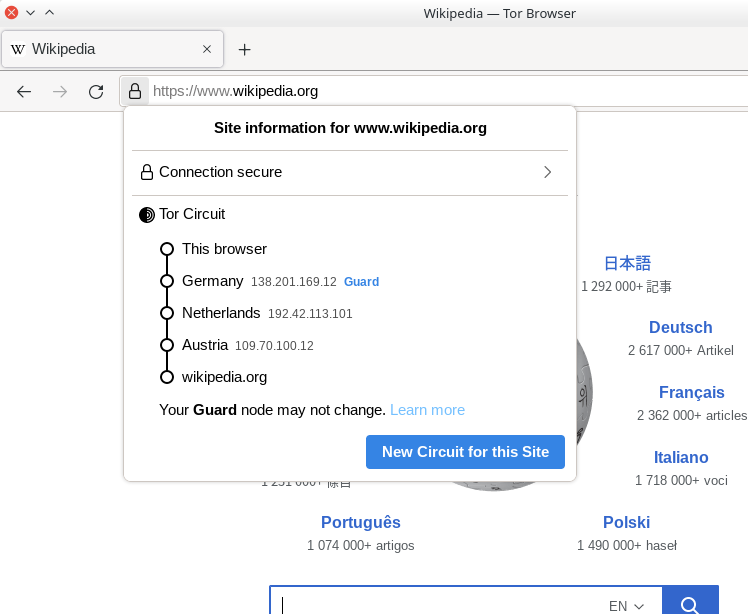
\includegraphics[width=.7\textwidth]{img/tor}
  \end{figure}
\end{myframe}
